\section{Durchführung}
\label{sec:Durchführung}

\subsection{Aufbau}
\subsubsection{Schlauchsystem und Prismen}
Für den Veruschsaufbau wird ein ringförmiges Schlauchsystem aus transparenten Schläuchen verwendet. An drei Stellen des Rings gibt es ausgedehnte, gerade Strecken aus einem härteren
Material. Die drei Abschnitte sind äquidistant verteilt, etwa $\SI{50}{\centi\meter}$ lang, ebenfalls transparent und besitzen verschiedene Durchmesser (je $\SI{10}{\milli\meter}$, 
$\SI{15}{\milli\meter}$ und $\SI{20}{\milli\meter}$). An einer anderen Stelle ist eine elektrische Zentrifugalpumpe in dem System integriert, über die die Strömungsgeschwindigkeit
eingestellt werden kann. Die Einstellungsmöglichkeiten reichen von \texttt{800 rpm} bis \texttt{9200 rpm}.

Für jeden geraden Schlauchabschnitt gibt es je ein Prisma, das durch eine passende Wölbung genau auf den Schlauch gelegt werden kann. Über einen Spalt unter der Wölbung kann das Prisma
am Schlauch festgeklemmt werden. Die Acrylprismen haben drei verschiedene, glatt geschliffene Oberflächen, dessen Flächennormalen je unterschiedlich zur Hauptachse zeigen.
Dadurch werden alle Strahlengänge auf diesen Winkel normiert. Die Winkel sind je 15°, 30° und 45°.
Der reale Versuchsaufbau ist in Abbildung \ref{fig:real} zu sehen.

\begin{figure}
    \centering
    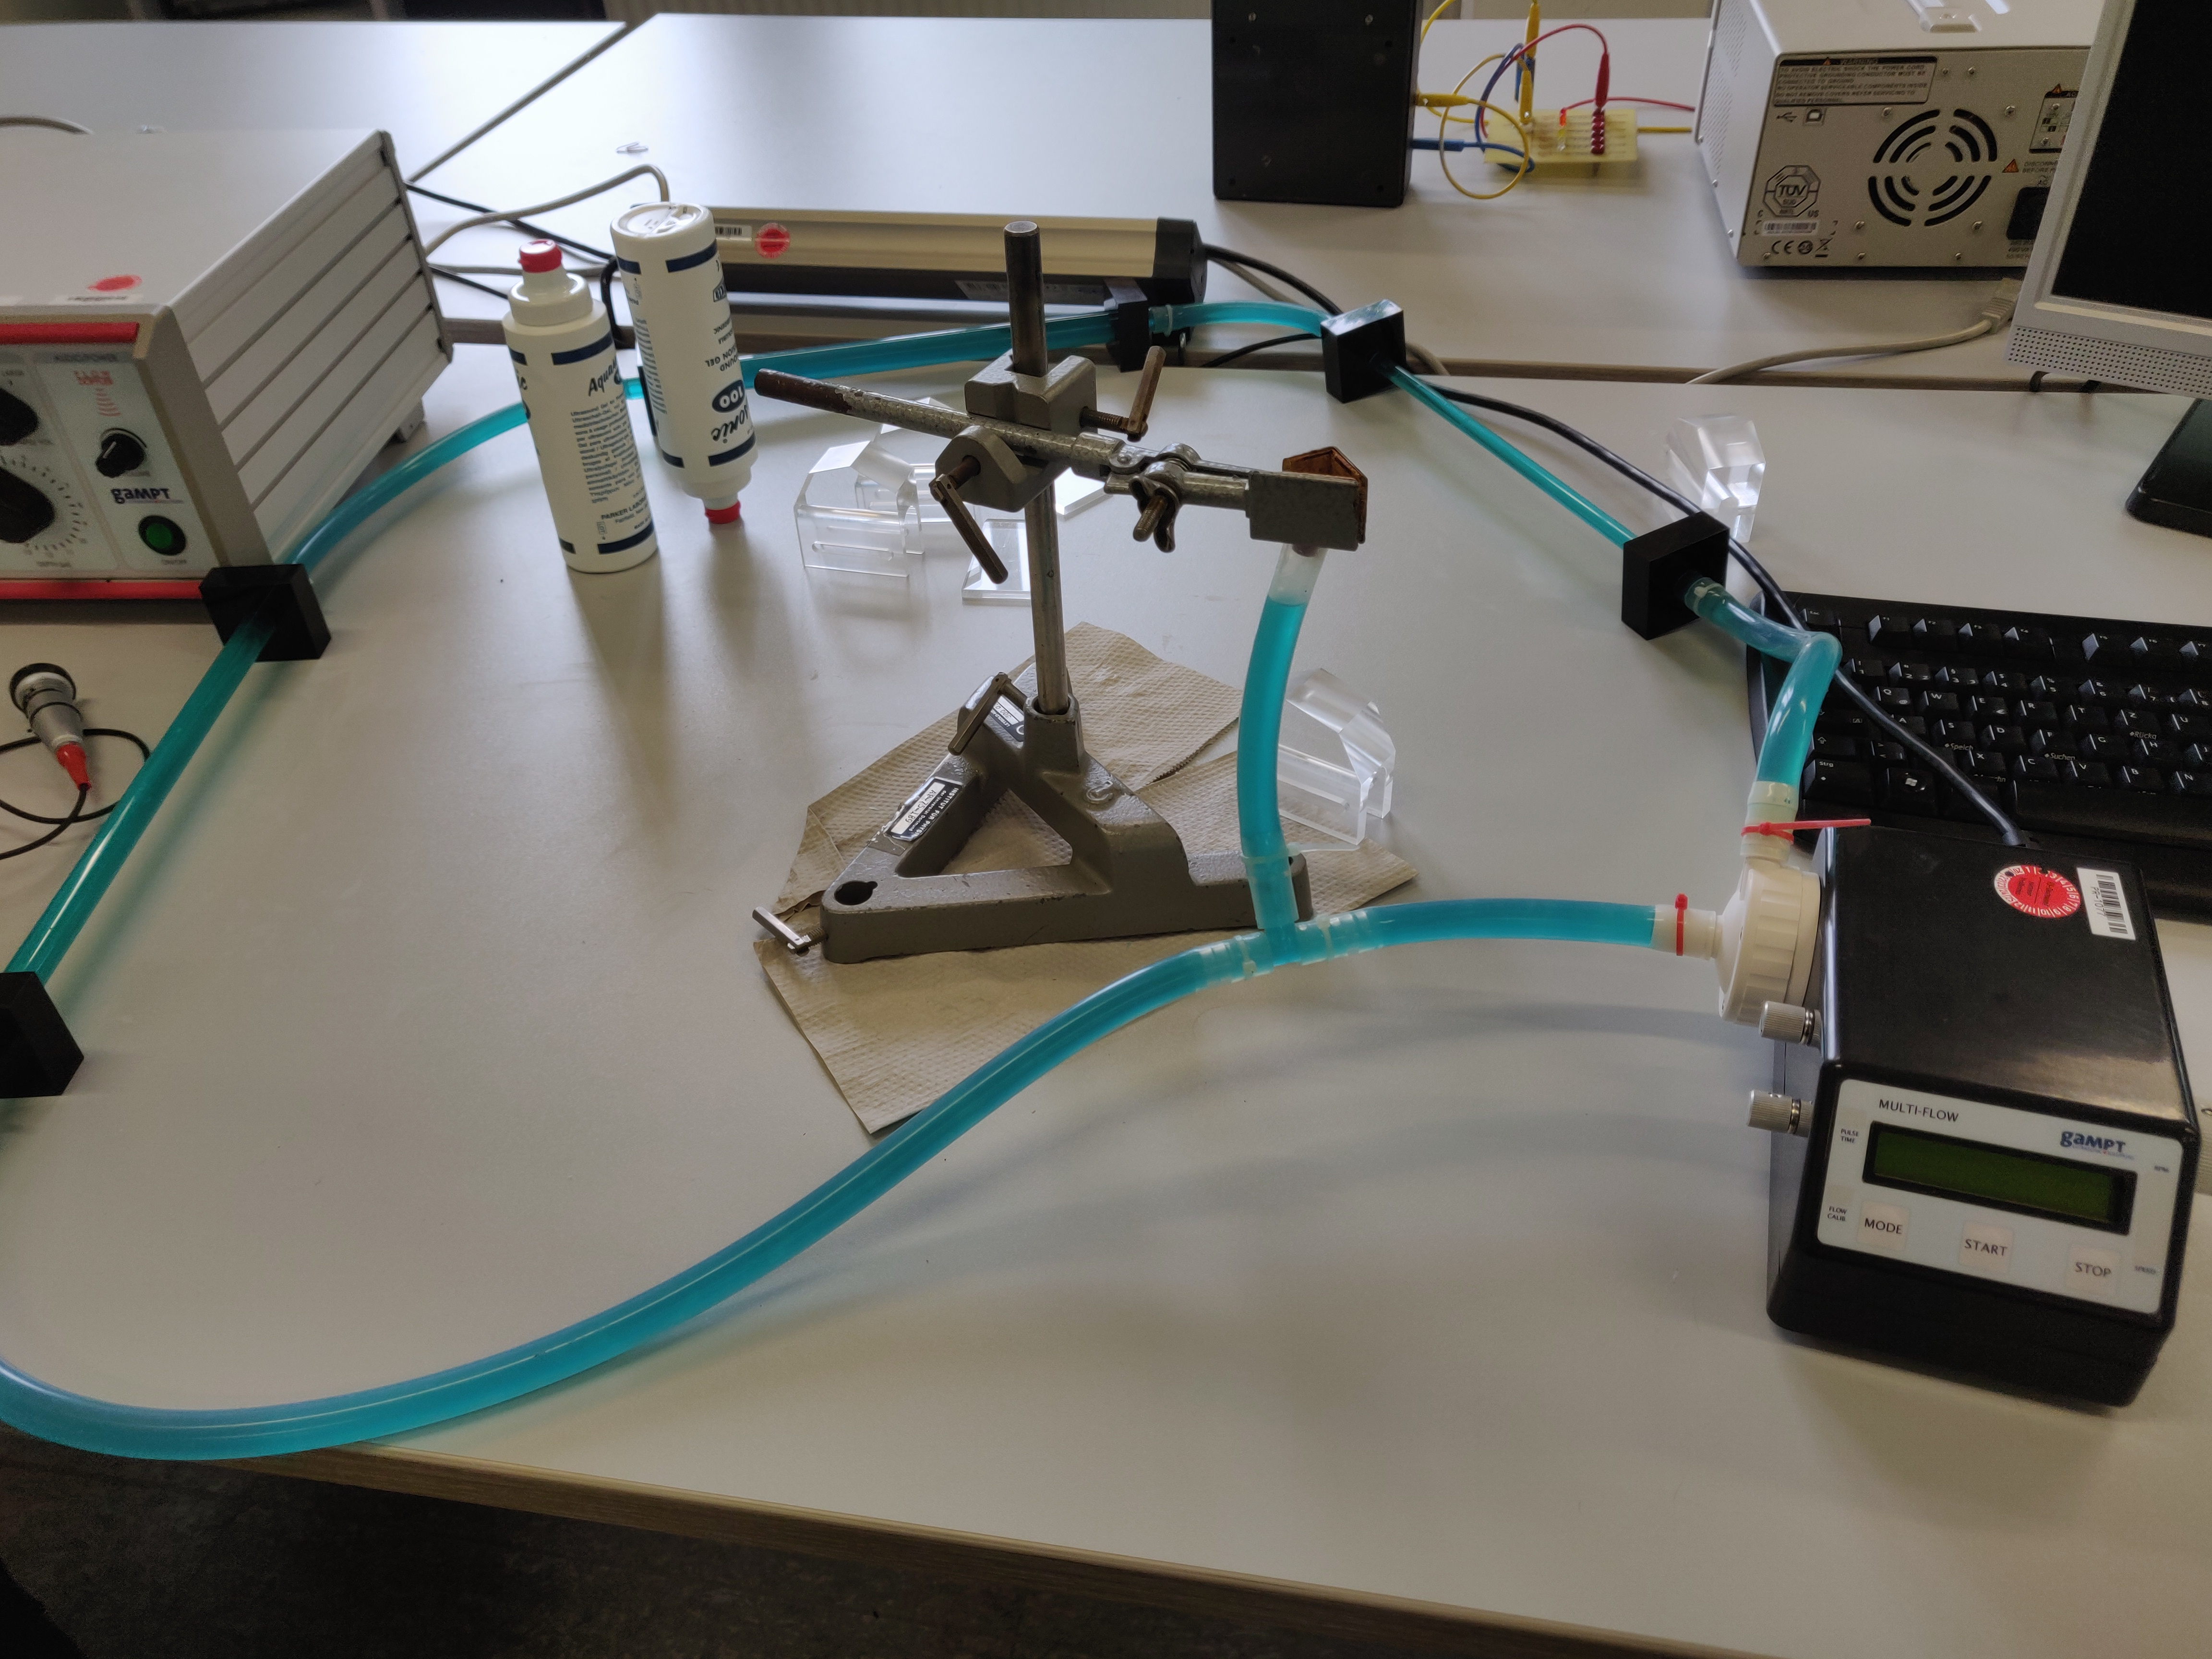
\includegraphics[width=.8\textwidth]{media/Schlauchsystem.jpg}
    \caption{Realer Veruschsaufbau des Schlauchrings.}
    \label{fig:real}
\end{figure}

\begin{figure}
    \centering
    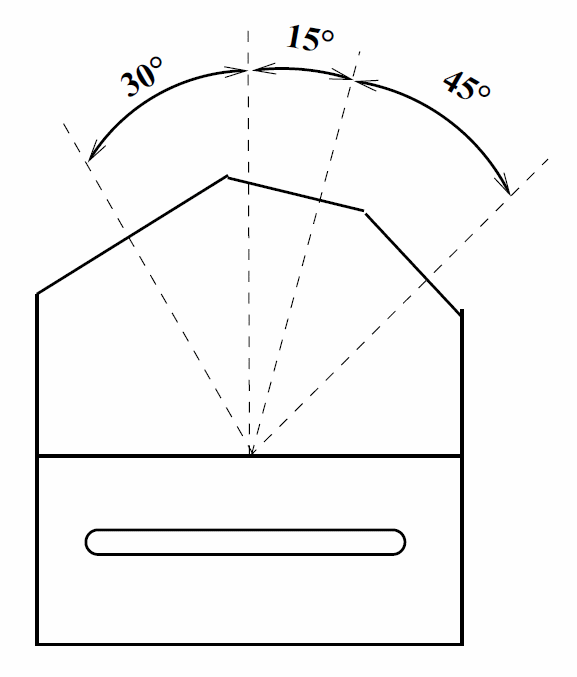
\includegraphics[width=.35\textwidth]{media/prisma.png}
    \caption{Schematische Darstellung eines Prismas. \cite{Versuchsanleitung}}
    \label{fig:prisma}
\end{figure}

\subsubsection{Ultraschall-Sonograph}
Für die Aufnahme von Messwerten wird ein Ultraschall-Sonograph verwendet. Dieser besteht aus einer Sonde, welche gleichzeitig Ultraschall-Wellen entsenden und empfangen kann.
Der für diesen Versuch verwendete Sonograph ist in Abbildung \ref{fig:sono} dargestellt.
Es können verschiedene Eindringtiefen durch zeitversetztes Senden \& Empfangen eingestellt werden. Außerdem gibt es diverse Stärkeregelungen und Signalverstärkemöglichkeiten.

Der Sonograph ist an einem Computer angeschlossen, auf dem ein Programm zum Auslesen der Daten installiert ist. Über das Programm lassen sich die verschiedenen Charakteristika
der empfangenen Wellen bestimmen, wie etwa Signalstärke und Frequenzunterschied.

\begin{figure}
    \centering
    \includegraphics[width=.8\textwidth][angle=-90]{media/Sonograph.jpg}
    \caption{Ultraschall-Sonograph.}
    \label{fig:sono}
\end{figure}

\subsection{Bestimmung der Strömungsgeschwindigkeit}
Für diese Messreihe wird die \texttt{SAMPLE VOLUME} des Sonographen auf \texttt{LARGE} und die Frequenz der Sonde auf $\SI{2}{\mega\hertz}$ gestellt.
Anschließend wird ein Prisma an einer der drei Abschnitte befestigt. Bei der Befestigung wird etwas Ultraschall-Gel auf das Rohr gegeben.
Es folgen Messungen aller drei Winkel bei fünf verschiedenen Strömungsgeschwindigkeiten, die über die Zentrifugalpumpe willkürlich eingestellt werden.
Dabei sollten zu hohe Drehzahlen vermieden werden, um turbulente Strömungen zu meiden.
Es wird etwas Ultraschall-Gel auf die Sonde gegeben und an diese dann auf Flächen des Prismas gedrückt. An dem Programm werden Signalstärke und Frequenzverschiebung abgelesen.

\subsection{Bestimmung des Strömungsprofils}
Diese Messungen werden an dem Schlauchabschnitt mit dem Durchmesser $\SI{15}{\milli\meter}$ und bei einem Doppler-Winkel von 15° durchgeführt. Die \texttt{SAMPLE VOLUME} wird auf \texttt{SMALL}
gestellt. In beiden Messreihen wird die Pumpleistung konstant gehalten bei je $70\%$ und $45\%$. Zu jeder Pumpleistung wird die Eindringtiefe von $\SI{12}{\micro\second}$ bis $\SI{19}{\micro\second}$
in $\SI{0.5}{\micro\second}$ Schritten eingestellt. Zu jedem Wert wird die Strömungsgeschwindigkeit und die Streuintensität gemessen.